\chapter{Functions of Two Variables}

In Chapter~\SS\ref{chap:Functions}, we learnt that functions can be described as a machine that takes in an input and produces an output according to a rule. Some examples of functions that we have encountered thus fare are $f(x) = x^2$, $g(x) = \cos x$, etc. These are functions of one variable, also called \vocab{univariate functions}.

However, in real life, there are functions that depend on more than one variable (i.e. the domain is not a subset of the real numbers). For instance, the cost (output) of a taxi ride may depend on variables (input) like time, distance travelled, traffic conditions, demand, etc. In this case, the function is called a \vocab{multivariate function}. The input with many variables can be expressed as a vector. 

Similarly, the codomain of a function does not necessarily need to be a subset of the real numbers. Consider the following function $f(s, t)$: \[f(s, t) = \cveciii{s + t}{t}{2s - 1}.\] Here, $f(s, t)$ takes in two inputs ($s$ and $t$), and spits out three outputs ($s + t$, $t$ and $2s - 1$).

For the rest of this chapter, we will only study scalar-valued functions of two variables, of the form \[z = f(x, y),\] which we can visualize in 3D space. We will see how the ideas from univariate functions can be extended to two variable functions and how concepts of vectors can be useful in studying these functions.

\section{Functions of Two Variables and Surfaces}

\subsection{Functions of Two Variables}

\begin{definition}
    A (scalar) \vocab{function of two variables}, $f$, is a rule that assigns each ordered pair of real numbers $(x, y)$ in its domain to a unique real number.
\end{definition}

Recall that the domain of a function $g(x)$ is a subset of the real number line, i.e. $\dom g \subseteq \RR$. Generalizing this to scalar functions of two variables, the domain of $f$ is a subset of the $xy$-plane, denoted $\RR \crossp \RR$ or $\RR ^2$. Mathematically, \[\dom f \subseteq \RR^2.\]

If the domain of $f(x, y)$ is not well specified, then we will take its domain to be the set of all pairs $(x, y) \in \RR^2$ for which the given expression is a well-defined real number.

\begin{example}[Domain of $f(x, y)$]
    Let $f(x, y) = \ln{y^2 - x}$. For $f(x, y)$ to be well-defined, the argument of the natural logarithm must be positive. That is, we require $y^2 - x > 0$. The domain of $f$ is hence \[\dom f = \bc{(x, y) \in \RR^2 \mid y^2 - x > 0}.\]
\end{example}

\subsection{Surfaces}

Recall that we defined the graph of a function $g(x)$ to be the collection of all points $(x, y)$ in the $xy$-plane such that the values $x$ and $y$ satisfy $y = g(x)$. We can extend this notion to functions of two variables:

\begin{definition}
    The \vocab{graph} of $z = f(x, y)$, or \vocab{surface} with equation $z = f(x, y)$, is the collection of all points $(x, y, z)$ in 3D Cartesian space such that the values $x$, $y$ and $z$ satisfy $z = f(x, y)$.
\end{definition}

Visualizing and illustrating a 3D surface can be challenging, especially as surfaces become complicated. We can study the surface by fixing or changing the variables one at a time. This is the idea behind traces, or level curves.

\begin{definition}
    \vocab{Horizontal traces} (or \vocab{level curves}) are the resulting curves when we intersect the surface $z = f(x, y)$ with horizontal planes.
\end{definition}

This is like fixing the value of $z$, giving the 2D graph of the equation $f(x, y) = c$ for some constant $c$.

\begin{definition}
    \vocab{Vertical traces} are the resulting curves when we intersect the surface $z = f(x, y)$ with vertical planes.
\end{definition}

This is like fixing the value of $x$ or $y$ (or a combination of both, e.g. $y = x$).

\begin{definition}
    A \vocab{contour plot} of $z = f(x, y)$ is a graph of numerous horizontal traces $f(x, y) = c$ for representative values of $c$ (usually spaced-out values).
\end{definition}

We may identify a surface by examining these traces to visualize graphs of two variables.

\begin{example}[Graph of $z = f(x, y)$]
    Let $f(x, y) = \ln{x^2 + y^2}$. Consider the horizontal traces of $z = f(x, y)$. Setting $z = c$, we get \[\ln{x^2 + y^2} = c \implies x^2 + y^2 = \e^c.\] Hence, the horizontal trace of $z = f(x, y)$ at $z = c$ corresponds to a circle centred at the origin with radius $\e^c$. Thus, the graph of $z = \ln{x^2 + y^2}$ looks like

    \begin{figure}[H]\tikzsetnextfilename{378}
        \centering
        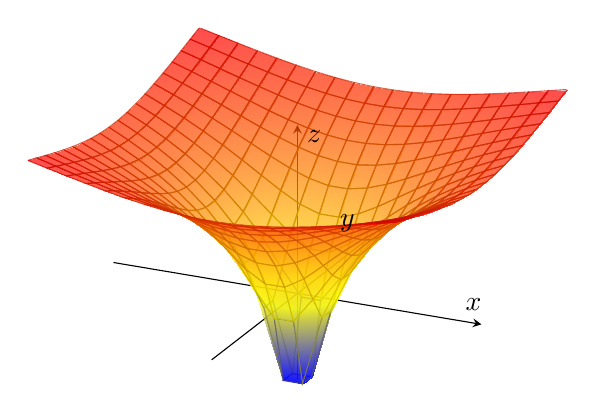
\begin{tikzpicture}[trim axis left, trim axis right]
            \begin{axis}[
                axis y line=middle,
                axis x line=middle,
                axis z line=middle,
                xtick = \empty,
                ytick = \empty,
                ztick = \empty,
                xlabel = {$x$},
                ylabel = {$y$},
                zlabel = {$z$},
                samples=20,
                ]
                \addplot3[surf,shader=faceted interp, colormap/hot,opacity=0.7, ]{ln(x^2 + y^2)};
            \end{axis}
        \end{tikzpicture}
        \caption{}
    \end{figure}
\end{example}

\subsection{Cylinders and Quadric Surfaces}

Exploring the traces of a surface allows us to visualize the shape of the surface. We can now look at some of the common surfaces, such as cylinders and quadric surfaces.

\begin{definition}
    A surface is a \vocab{cylinder} if there is a plane $P$ such that all planes parallel to $P$ intersect the surface in the same curve (when viewed in 2D).
\end{definition}

Examples of cylinders include the graphs of $x^2 + z^2 = 1$ and $z = y^2$, as shown below:

\begin{figure}[H]
    \centering
    \begin{minipage}[t]{.5\textwidth}\tikzsetnextfilename{379}
      \centering
      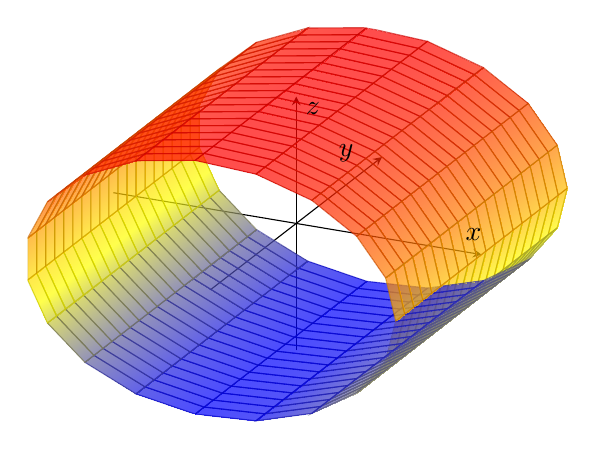
\begin{tikzpicture}[trim axis left, trim axis right]
        \begin{axis}[
            axis y line=middle,
            axis x line=middle,
            axis z line=middle,
            xtick = \empty,
            ytick = \empty,
            ztick = \empty,
            xlabel = {$x$},
            ylabel = {$y$},
            zlabel = {$z$},
            samples=20,
            ]
            \addplot3[surf,shader=faceted interp, colormap/hot,opacity=0.7,y domain=0:2*pi] ({cos(deg(y))},{x},{sin(deg(y))});
        \end{axis}
        \end{tikzpicture}
      \captionof{figure}{Graph of $x^2 + z^2 = 1$.}
    \end{minipage}%
    \begin{minipage}[t]{.5\textwidth}\tikzsetnextfilename{380}
      \centering
      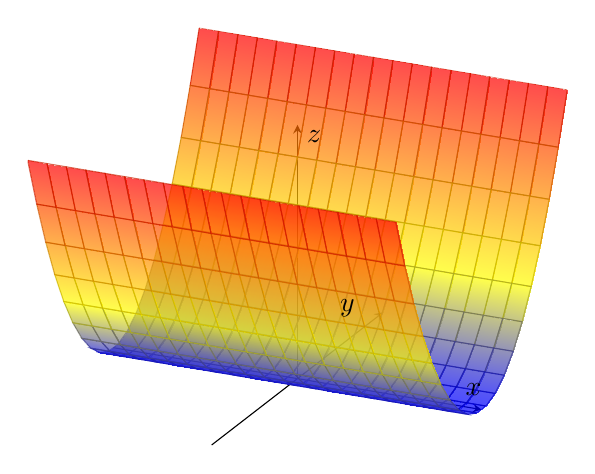
\begin{tikzpicture}[trim axis left, trim axis right]
        \begin{axis}[
            axis y line=middle,
            axis x line=middle,
            axis z line=middle,
            xtick = \empty,
            ytick = \empty,
            ztick = \empty,
            xlabel = {$x$},
            ylabel = {$y$},
            zlabel = {$z$},
            samples=20,
            ]
            \addplot3[surf,shader=faceted interp, colormap/hot,opacity=0.7, ] {y^2};
        \end{axis}
        \end{tikzpicture}
      \captionof{figure}{Graph of $z = y^2$.}
    \end{minipage}
\end{figure}

Observe that $x^2 + z^2 = 1$ is a special case of a function of two variables $z = f(x, y)$ that can be reduced to $z = f(x)$ since $z$ is independent of $y$. Similarly, $z = y^2$ can be reduced to $z = f(y)$ since $z$ is independent of $x$. Indeed, if a function $z = f(x, y)$ can be reduced to a univariate function, then its surface must be cylindrical.

Another common surface is a quadric surface, which is a 3D generalization of 2D conic sections. Recall that a conic section in 2D has the general form \[Ax^2 + Bxy + Cy^2 + Dx + Ey + F = 0.\] We can generalize this into 3D to get a quadric surface.

\begin{definition}
    A \vocab{quadric surface} has the form \[Ax^2 + By^2 + Cz^2 + Dxy + Eyz + Fzx + Gx + Hy + Iz + J,\] where $A, B, \dots, J \in \RR$ and at least one of $A$, $B$ and $C$ is non-zero.
\end{definition}

An example of a quadric surface is the ellipsoid, which is a generalization of an ellipse and has equation \[\frac{x^2}{a^2} + \frac{y^2}{b^2} + \frac{z^2}{c^2} = 1.\]

\begin{figure}[H]\tikzsetnextfilename{381}
    \centering
    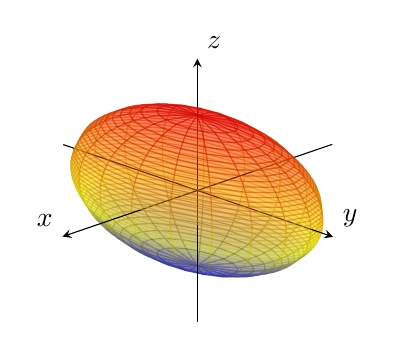
\begin{tikzpicture}
        \begin{axis}
        [view={135}{20},%colormap/blackwhite,
        axis lines=center, axis on top,ticks=none,
        set layers=default,axis equal,
        xlabel={$x$}, ylabel={$y$}, zlabel={$z$},
        xlabel style={anchor=south east},
        ylabel style={anchor=south west},
        zlabel style={anchor=south west},
        enlargelimits,
        tick align=inside,
        domain=0:2.00,
        samples=20, 
        z buffer=sort,
        ]
        \addplot3 [surf,opacity=0.4,domain=-1:0,
        domain y=0:360] ({sin(y)*sqrt(1-x^2)},{2*cos(y)*sqrt(1-x^2)},{x});
        \addplot3 [surf,opacity=0.4,domain=0:1,
        domain y=0:360,on layer=axis foreground] ({sin(y)*sqrt(1-x^2)},{2*cos(y)*sqrt(1-x^2)},{x});
        \end{axis}
    \end{tikzpicture}
    \caption{An ellipsoid.}
\end{figure}

When $a = b = c = r$, we get the equation \[x^2 + y^2 + z^2 = r^2.\] This represents a sphere centred at the origin with radius $r$. Observe the similarity between the equation of a circle ($x^2 + y^2 = r^2$) and the equation of a sphere.

\section{Partial Derivatives}

Recall that for a function $f$ of one variable $x$, we defined the derivative function as \[f'(x) = \lim_{\D x \to 0} \frac{f(x + \D x) - f(x)}{\D x}.\] The usual notations are $\der{y}{x}$ or $\der{f}{x}$ if $y = f(x)$.

The notation $\der{y}{x}$ gives some insight into how derivatives are derived. We can view
\begin{itemize}
    \item ``$\d x$'' as a small change in $x$, and
    \item ``$\d y$'' as the change in $y$ as a result of the small change in $x$.
\end{itemize}
Hence, the notation $\der{y}{x}$ actually represents the ``rise over run'', which is a measure of gradient at the point $(x, y)$ on the graph.

We can extend this notion to functions of two variables $z = f(x, y)$. There are now two variables that will affect the change in the value of $f$. We can choose to vary $x$ slightly ($\D x$) or vary $y$ slightly $\D y$ and see how $f$ changes ($\D f$). This gives us some notion of a derivative. However, because we are only varying one independent variable at a time, we are only differentiating the function $f(x,y)$ ``partially''. We hence call these derivatives the partial derivatives of $f$.

\begin{definition}
    The (first-order) \vocab{partial derivatives} of $f(x, y)$ are the functions $f_x$ and $f_y$ defined by
    \begin{align*}
        f_x(x, y) &= \lim_{\D x \to 0} \frac{f(x + \D x, y) - f(x, y)}{\D x},\\
        f_y(x, y) &= \lim_{\D y \to 0} \frac{f(x, y + \D y) - f(x, y)}{\D y}.
    \end{align*}
    In Liebniz notation, \[f_x(x, y) = \pder{f}{x}, \quad f_y(x, y) = \pder{f}{y}.\]
\end{definition}

\begin{recipe}[Partial Differentiation]
    To partially differentiate a function $f(x, y)$ with respect to $x$, we differentiate $f(x, y)$ as we normally would, treating $y$ as a constant. Similarly, if we are partially differentiating with respect to $y$, we treat $x$ as a constant.
\end{recipe}

\begin{sample}
    Given $f(x, y) = \cos{xy + y^2}$, find $f_x(x, y)$.
\end{sample}
\begin{sampans}
    To partially differentiate it with respect to $x$, we treat $y$ as a constant. Using the chain rule, \[f_x (x, y) = -\sin{xy + y^2} \, \pder{}{x} \bs{xy + y^2}.\] Since $y$ is a constant, \[\pder{}{x} (xy) = y, \quad \pder{}{x} y^2 = 0.\] Hence, \[f_x (x, y) = -y\sin{xy + y^2}.\]
\end{sampans}

\subsection{Geometric Interpretation}\label{subsec:Partial-Derivative-Geometric}

Consider a surface $S$ given by the equation $z = f(x, y)$. Let $P(a, b, c)$ be a point on $S$.

\begin{figure}[H]
    \centering
    \includegraphics[scale=0.5]{media/partial derivative.png}
    \caption{Partial derivatives as slopes of tangent lines.\protect\footnotemark}
\end{figure}
\footnotetext{Source: \url{https://www2.victoriacollege.edu/~myosko/m2415sec143notes(7).pdf}}

The curve $C_1$ is the graph of the function $g(x) = f(x, b)$, which is the intersection curve of the surface and the vertical plane $y = b$. The slope of its tangent $T_1$ at $P$ is $g'(x) = f_x(a, b)$.

Similarly, the curve $C_2$ is the graph of the function $h(y) = f(a, y)$, which is the intersection curve of the surface and the vertical plane $x = a$. The slope of its tangent $T_2$ at $P$ is $h'(y) = f_y(a, b)$.

We can hence visualize partial derivatives at the point $P$ on $S$ as slopes to the tangent lines $T_1$ and $T_2$ at that point.

\subsection{Gradient}

To represent the ``full'' derivative of a function, we simply collect its partial derivatives.

\begin{definition}
    The \vocab{gradient} of a function $f(x, y)$, denoted as $\nabla f$, is the collection of all its partial derivatives into a vector. \[\nabla f = \cvecii{f_x}{f_y}.\]
\end{definition}

\begin{example}[Gradient]
    Let $f(x, y) = xy^2 + x^3$. Then its gradient is \[\nabla f = \cvecii{f_x}{f_y} = \cvecii{y^2 + 3x^2}{2xy}.\]
\end{example}

\subsection{Second Partial Derivatives}

Similar to second-order derivatives for univariate functions, we can also consider the partial derivatives of partial derivatives: \[(f_x)_x, \quad (f_x)_y, \quad (f_y)_x, \quad (f_y)_y.\] If $z = f(x, y)$, we use the following notation for the second partial derivatives:
\[
    \begin{array}{c @{{}={}} >{\displaystyle} c @{{}={}} >{\displaystyle} c}
        (f_x)_x = f_{xx} & \pder[2]{f}{x} & \pder[2]{z}{x},\\[0.5cm]
        (f_x)_y = f_{xy} & \frac{\partial^2 f}{\partial y \, \partial x} & \frac{\partial^2 z}{\partial y \, \partial x},\\[0.5cm]
        (f_y)_x = f_{yx} & \frac{\partial^2 f}{\partial x \, \partial y} & \frac{\partial^2 z}{\partial x \, \partial y},\\[0.5cm]
        (f_y)_y = f_{yy} & \pder[2]{f}{y} & \pder[2]{z}{y}.
    \end{array}
\]
Thus, the notation $f_{xy}$ means that we first partially differentiate with respect to $x$ and then with respect to $y$. Notice that the order the variables appear in the denominator is reversed when using Liebniz notation, similar to the idea of composite functions: \[(f_x)_y = \pder{}{y} \bp{\pder{f}{x}} = \frac{\partial^2 f}{\partial y \, \partial x}.\]

\begin{example}[Second Partial Derivatives]
    Consider the function $f(x, y) = xy^2 + x^3 + \ln y$. Its partial derivatives are \[f_x = y^2 + 3x^2, \quad f_y = 2xy + \frac1y,\] and its second partial derivatives are \[f_{xx} = 6x, \quad f_{xy} = 2y, \quad f_{yx} = 2y, \quad f_{yy} = 2x  - \frac1{y^2}.\]
\end{example}

Notice in the above example that $f_{xy} = f_{yx}$. This symmetry of second partial derivatives is known as Clairaut's theorem.

\begin{theorem}[Clairaut's Theorem]
    If $f_{xy}$ and $f_{yx}$ are both continuous, then $f_{xy} = f_{yx}$
\end{theorem}

\subsection{Multivariate Chain Rule}\label{subsec:Multivariate-Chain-Rule}

Recall that for a univariate function $y = f(x)$, where the variable $x$ is a function of $t$, i.e. $x = g(t)$, the chain rule states \[\der{y}{t} = \der{y}{x} \der{x}{t}.\] We can generalize this result to multivariate functions using partial derivatives:

\begin{proposition}[Multivariate Chain Rule]
    Consider the function $f(x, y)$, where $x$ and $y$ are functions of $t$. Then \[\der{f}{t} = \pder{f}{x} \der{x}{t} + \pder{f}{y} \der{y}{t}.\]
\end{proposition}

To see why this is morally true, we return to the definition of a partial derivative:
\begin{align*}
    f_x(x, y) &= \lim_{\D x \to 0} \frac{f(x + \D x, y) - f(x, y)}{\D x},\\
    f_y(x, y) &= \lim_{\D y \to 0} \frac{f(x, y + \D y) - f(x, y)}{\D y}.
\end{align*}
Rewriting these equations, we get
\begin{align*}
    f(x + \D x, y) &= f(x, y) + \D x f_x(x, y), \tag{1}\\
    f(x, y + \D y) &= f(x, y) + \D y f_y(x, y), \tag{2}
\end{align*}
where $\D x$ and $\D y$ should be thought of as infinitesimally small changes in $x$ and $y$.

We now consider the quantity $f(x + \D x, y + \D y)$. Applying (1) and (2) sequentially, we get
\begin{align*}
    f(x + \D x, y + \D y) &= f(x, y + \D y) + \D x f_x(x, y + \D y)\\
    &= f(x, y) + \D y f_y(x,y) + \D x f_x(x, y + \D y). \tag{3}
\end{align*}
Observe that if we partially differentiate (2) with respect to $x$, we get \[f_x(x, y + \D y) = f_x(x, y) + \D y f_{yx}(x, y).\] Substituting this into (3) yields
\begin{align*}
    f(x + \D x, y + \D y) &= f(x, y) + \D y f_y(x,y) + \D x \bs{f_x(x, y) + \D y f_{yx}(x, y)}\\
    &= f(x, y) + \D y f_y(x,y) + \D x f_x(x, y) + \D x\D y f_{yx}(x, y). \tag{4}
\end{align*}
Since $\D x$ and $\D y$ are both infinitesimally small, the quantity $\D x \D y$ is negligible and can be disregarded. We thus have \[\D f = f(x + \D x, y + \D y) - f(x, y) = \D x f_x(x, y) + \D y f_y(x,y).\] Dividing throughout by $\D t$ and writing $f_x$, $f_y$ in Liebniz notation, we have \[\frac{\D f}{\D t} = \pder{f}{x} \frac{\D x}{\D t} + \pder{f}{y} \frac{\D y}{\D t}.\] In the limit as $\D t \to 0$, we have \[\frac{\D f}{\D t} \to \der{x}{t}, \quad \frac{\D x}{\D t} \to \der{x}{t}, \quad \frac{\D y}{\D t} \to \der{y}{t}.\] Thus, \[\der{f}{t} = \pder{f}{x} \der{x}{t} + \pder{f}{y} \der{y}{t}.\] \qed

Observe that if we had applied (2) before (1) on $f(x + \D x, y + \D y)$, we would have got \[f(x + \D x, y + \D y) = f(x, y) + \D y f_y(x,y) + \D x f_x(x, y) + \D x\D y f_{xy}(x, y).\] However, by Clairaut's theorem, we know $f_{xy} = f_{yx}$, so we would still have ended up with (4).

\subsection{Directional Derivative}

So far, we only know how to find the instantaneous rate of change of $f(x, y)$ in two special cases:
\begin{itemize}
    \item The first case is when we vary $x$ and hold $y$ constant, in which the partial derivative $f_x(x, y)$ represents the instantaneous rate of change of $f(x, y)$.
    \item The second case is when we vary $y$ and hold $x$ constant, in which the partial derivative $f_y(x, y)$ represents the instantaneous rate of change of $f(x, y)$.
\end{itemize}
We wish to construct a more general ``derivative'' which represents the instantaneous rate of change of $f(x, y)$ where $x$ and $y$ are both allowed to vary.

To simplify matters, we assume that $x$ and $y$ are changing at a constant rate. That is, every time $x$ increases by $u_x$, $y$ will increase by $u_y$. We can represent this change with a unit vector $\vec u$ along the $xy$-plane: \[\vec u = \cvecii{u_x}{u_y}.\] Because we are measuring the instantaneous rate of change of $f(x, y)$ along a direction, we call this quantity the ``directional derivative''.

\begin{definition}
    The \vocab{directional derivative} of $f(x, y)$ in the direction of the unit vector $\vec u = \cveciix{u_x}{u_y}$ is denoted $D_{\vec u} f(x, y)$ and is defined as \[D_{\vec u} f(x, y) = \lim_{h \to 0} \frac{f(x + h u_x, y + h u_y) - f(x, y)}{h}.\]
\end{definition}

We now relate the directional derivative with the gradient of $f$.

\begin{proposition}
    \[D_{\vec u} f(x, y) = \nabla f \cdot \vec u = u_x f_x(x, y) + u_y f_y (x, y).\]
\end{proposition}
\begin{proof}
    In \SS\ref{subsec:Multivariate-Chain-Rule}, we derived the equation \[f(x + \D x, y + \D y) - f(x, y) = \D x f_x(x, y) + \D y f_y(x, y),\] where $\D x$ and $\D y$ are infinitesimally small. If we take $\cveciix{\D x}{\D y}$ to be in the same direction as $\cveciix{u_x}{u_y}$, i.e. \[\cvecii{\D x}{\D y} = \lim_{h \to 0} h \cvecii{u_x}{u_y},\] then we have \[f(x + h u_x, y + h u_y) - f(x, y) = h u_x f_x(x, y) + h u_y f_y(x, y),\] keeping in mind that we are taking the limit $h \to 0$ on both sides. Dividing both sides throughout by $h$, \[\lim_{h \to 0} \frac{f(x + h u_x, y + h u_y) - f(x, y)}{h} = u_x f_x(x, y) + u_y f_y(x, y),\] which was what we wanted.
\end{proof}

With this relation, we can prove several neat results.

\begin{proposition}
    Suppose $f$ is differentiable at $(x_0, y_0)$, and $\nabla f(x_0, y_0) \neq \vec 0$. Then $\nabla f(x_0, y_0)$ is perpendicular to the level curve of $f$ through $(x_0, y_0)$.
\end{proposition}
\begin{proof}
    Let $f(x, y) = (x(t), y(t))$. Note that the tangent to the level curve at $(x_0, y_0)$ has direction vector $\vec u = \cveciix{\derx{x}{t}}{\derx{y}{t}}$.
    
    Let the level curve at $(x_0, y_0)$ have equation $f(x, y) = c$. Implicitly differentiating this with respect to $t$, we get \[\pder{f}{x} \der{x}{t} + \pder{f}{y} \der{y}{t} = \cvecii{f_x}{f_y} \dotp \cvecii{\derx{x}{t}}{\derx{y}{t}} = \nabla f \dotp \vec u = 0.\] Since both $\nabla f$ and $\vec u$ are non-zero vectors, they must be perpendicular to each other.
\end{proof}

\begin{proposition}
    The greatest rate of change of $f$ occurs in the direction of $\nabla f$, while the smallest rate of change occurs in the direction of $-\nabla f$
\end{proposition}
\begin{proof}
    Since $\vec u$ is a unit vector, \[D_{\vec u} f = \nabla f \dotp \vec u = \abs{\nabla f} \abs{\vec u} \cos \t = \abs{\nabla f} \cos \t,\] where $\t$ is the angle between $\nabla f$ and $\vec u$. Clearly, $D_{\vec u} f$ is maximal when $\t = 0$, in which case $\vec u$ is in the same direction as $\nabla f$. Similarly, $D_{\vec u} f$ is minimal when $\t = \pi$, in which case $\vec u$ is in the opposite direction as $\nabla f$.
\end{proof}

We say that $\nabla f(a,b)$ is the \vocab{direction of steepest ascent} at $(a, b)$, while $-\nabla f(a, b)$ is the \vocab{direction of steepest descent}.

\subsection{Implicit Differentiation}

Consider the unit circle, which has equation \[x^2 + y^2 = r^2.\] Previously, we learnt that to find $\derx{y}{x}$, we can simply differentiate term by term, treating $y$ as a function of $x$ and using the chain rule \[\der{}{x} g(y) = \der{}{y} g(y) \cdot \der{y}{x}.\] Using our example of the unit circle, we get \[2x + 2y \der{y}{x} = 0 \implies \der{y}{x} = -\frac{y}{x}.\] While morally true, this approach to implicit differentiate is not entirely rigorous. For a more formal justification, we turn to partial derivatives.

Going back to our example of the unit circle, if we move all terms to one side of the equation, we get \[x^2 + y^2 - r^2 = 0.\] Now, observe that the LHS is simply a function of $x$ and $y$, i.e. \[f(x, y) = x^2 + y^2 - r^2.\] Hence, we can define $y$ implicitly as a function of $x$ that satisfies \[f(x, y) = 0.\] If we differentiate the above equation with respect to $x$, by the multivariate chain rule, we get \[\der{f}{x} = \pder{f}{x} \der{x}{x} + \pder{f}{y} \der{y}{x} = 0.\] Clearly, $\derx{x}{x} = 1$. Rearranging, we get \[\der{y}{x} = -\frac{f_x(x, y)}{f_y(x, y)}.\] Since \[f_x(x, y) = 2x, \quad \tand \quad f_y(x, y) = 2y,\] we get \[\der{y}{x} = -\frac{2x}{2y} = -\frac{x}{y}\] as expected. 

More generally,
\begin{proposition}[Implicit Differentiation for Univariate Functions]
    If the equation \[f(x, y) = 0\] implicitly defines $y$ as a function of $x$, then \[\der{y}{x} = -\frac{f_x(x, y)}{f_y(x,  y)},\] given that $f_y(x, y) \neq 0$.
\end{proposition}

We can extend this result to functions of two variables.
\begin{proposition}[Implicit Differentiation for Functions of Two Variables]
    If the equation \[f(x, y, z) = 0\] implicitly defines $z$ as a function of $x$ and $y$, then \[\pder{z}{x} = -\frac{f_x(x, y, z)}{f_z(x,  y, z)} \quad \tand \quad \pder{z}{y} = -\frac{f_y(x, y, z)}{f_z(x, y, z),}\] given that $f_z(x, y, z) \neq 0$.
\end{proposition}

To see this in action, consider the following sample problem:

\begin{sample}
    Find the value of $\pderx[2]{z}{x}$ at $(0, 0, c)$ of the ellipsoid \[\frac{x^2}{a^2} + \frac{y^2}{b^2} + \frac{z^2}{c^2} = 1.\]
\end{sample}
\begin{sampans}
    Let \[f(x, y, z) = \frac{x^2}{a^2} + \frac{y^2}{b^2} + \frac{z^2}{c^2} - 1.\] Applying the above result, we have \[\pder{z}{x} = -\frac{f_x(x, y, z)}{f_z(x,  y, z)} = -\frac{2x / a^2}{2z / c^2} = -\frac{c^2}{a^2} \frac{x}{z}.\] Partially differentiating with respect to $x$ once more, \[\pder[2]{z}{x} = \pder{z}{x} \bp{-\frac{c^2}{a^2} \frac{x}{z}} = -\frac{c^2}{a^2 z}.\] Hence, \[\pder[2]{z}{x}{(0, 0, c)} = -\frac{c}{a^2}.\]
\end{sampans}

\section{Approximations}

In \SS\ref{chap:Maclaurin-Series}, we learnt that \[f(x) = f(0) + f'(0) x + \frac{f''(0)}{2!} x^2 + \frac{f^{(3)}(0)}{3!} x^3 + \dots.\]

If we want to approximate $f(x)$ for $x$ near $0$, we can truncate the Maclaurin series of $f(x)$. For instance, the linear approximation to $x$ is \[f(x) \approx f(0) + f'(0),\] which is the tangent line at $x = 0$. If we want better approximations, we can simply take more terms. For instance, if we take one more term, then we get the quadratic approximation \[f(x) \approx f(0) + f'(0) x + \frac{f''(0)}{2!} x^2.\]

In some sense, we can get a good approximation to $f(x)$ around $x = 0$ if we can find a simpler function which
\begin{itemize}
    \item has the same value as $f$ at $x = 0$, and
    \item has the same derivatives as $f$ at $x = 0$ (up to the order of derivatives we prefer).
\end{itemize}

The same idea is extended to functions of two variables (or any multivariate functions) at a general point. The idea of approximation $f(x, y)$ at a point $(a, b)$ is to find a simpler function which
\begin{itemize}
    \item has the same value as $f$ at $(a, b)$, and
    \item has the same $n$th-order partial derivatives as $f$ at $(a, b)$ (where $n$ is the highest order we prefer).
\end{itemize}

In this subsection, we look at the case where $n = 1$ (linear approximation) and $n = 2$ (quadratic approximation).

\subsection{Tangent Plane}

To find a linear approximation of $f(x, y)$ at $(a, b)$ is to find a simpler function which
\begin{itemize}
    \item has the same value as $f$ at $(a, b)$, and
    \item has the same partial derivatives as $f$ at $(a, b)$.
\end{itemize}
Let this approximation be $T(x, y)$. As the name suggests, $T(x, y)$ is linear and is hence of the form \[T(x, y) = C_1 + C_2 (x-a) + C_3 (y-b),\] where $C_1$, $C_2$ and $C_3$ are constants to be determined.

From the first condition, we require $f(a, b) = T(a, b)$. Hence, \[f(a, b) = T(a, b) = C_1.\]

From the second condition, we require $f_x(a, b) = T_x(a, b)$ and $f_y(a, b) = T_y(a, b)$. This gives \[f_x(a,b) = T_x(a,b) = C_2\] and \[f_y(a, b) = T_y(a,b) = C_3.\]

We hence have:
\begin{proposition}[Linear Approximation]
    The linear approximation at $(a, b)$ is given by \[T(x, y) = f(a, b) + f_x(a,b) (x-a) + f_y(a, b) (y-b).\]
\end{proposition}

Recall that the linear approximation to a univariate function at $x = a$ is the tangent line at that point. Generalizing this up a dimension, the linear approximation $T(x, y)$ is the \vocab{tangent plane} to $f(x, y)$ at $(a, b)$.

Using 3D vector geometry, we can find the normal vector to $z = f(x, y)$ at $(a, b)$: \[\vec n = \cveciii{f_x(a,b)}{f_y(a,b)}{-1}.\]

\subsection{Quadratic Approximation}

To find a quadratic approximation of $f(x, y)$ at $(a, b)$ is to find a simpler function which
\begin{itemize}
    \item has the same value as $f$ at $(a, b)$, and
    \item has the same first and second partial derivatives as $f$ at $(a, b)$.
\end{itemize}

\begin{remark}
    In univariate functions, the word ``quadratic'' refers to functions with terms of order 2, such as $x^2$. Similarly with multivariables, ``quadratic'' refers to terms with order 2, but it could be $x^2$, $y^2$ or $xy$; all variables contribute to the total order of the term. For instance, $x^2 y^3$ is a term of order $2 + 3 = 5$.
\end{remark}

To get the quadratic approximation $Q(x, y)$, we simply add terms of order 2 to the linear approximation $T(x, y)$: \[Q(x, y) =  T(x,y) + C_1 (x-a)^2 + C_2 (x-a)(y-b) + C_3 (y-b)^2,\] where $C_1$, $C_2$ and $C_3$ are constants. We can determine them by equating the second partial derivatives of $Q(x, y)$ with that of $f(x, y)$'s:
\begin{align*}
    f_{xx}(a, b) = Q_{xx}(a, b) &= 2C_1,\\
    f_{xy}(a, b) = Q_{xx}(a, b) &= \phantom{2}C_2,\\
    f_{yy}(a, b) = Q_{xx}(a, b) &= 2C_3.
\end{align*}

We hence have:
\begin{proposition}[Quadratic Approximation]
    The quadratic approximation at $(a, b)$ is given by
    \begin{align*}
        Q(x, y) &= f(a, b) + f_x(a, b) (x-a) + f_y(a, b) (y-b)\\
        &\hspace{2em} + \frac12 f_{xx}(a,b) (x-a)^2 + f_{xy}(a, b) (x-a)(y-b) + \frac12 f_{yy}(a, b) (y-b)^2.
    \end{align*}
\end{proposition}

Note that by Clairaut's theorem, we can interchange $f_{xy}$ and $f_{yx}$ in the formula above, so long as they are continuous.

\section{Maxima, Minima and Saddle Points}

One important application of calculus is the optimization of functions which have many dependent variables. For example, one may maximize the amount of profit based on parameters such as the cost of raw materials, workers' salaries, time needed for production, etc.

To find stationary points of a univariate function, we equate its gradient to 0. Similarly, for functions of two variables $f(x, y)$, if we want to find stationary points, we look for points where its gradient, $\nabla f$, is the zero vector, i.e. \[\nabla f = \cvecii{f_x}{f_y} = \cvecii00.\]

In functions of two variables, the stationary points we often come across are maxima, minima and saddle points (so named because it looks like a horse saddle).

\begin{figure}[H]
    \centering
    \begin{minipage}[t]{.5\textwidth}\tikzsetnextfilename{383}
      \centering
      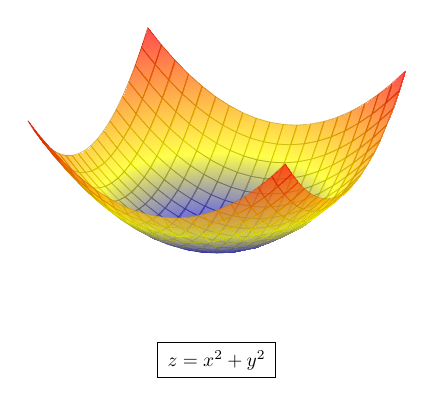
\begin{tikzpicture}[scale=0.7,trim axis left, trim axis right]
        \begin{axis}[
            hide axis,
            samples=20,
            legend cell align={left},
            legend style={at={(0.5, -0.05)},anchor=north},
            ]
            \addplot3[surf,shader=faceted interp, colormap/hot,opacity=0.7,domain=-1:1,y domain=-1:1,empty legend] {x^2 + y^2};
            \addlegendentry{$z = x^2 + y^2$};
        \end{axis}
        \end{tikzpicture}
      \captionof{figure}{Minimum point at $(0, 0)$.}
    \end{minipage}%
    \begin{minipage}[t]{.5\textwidth}\tikzsetnextfilename{384}
      \centering
      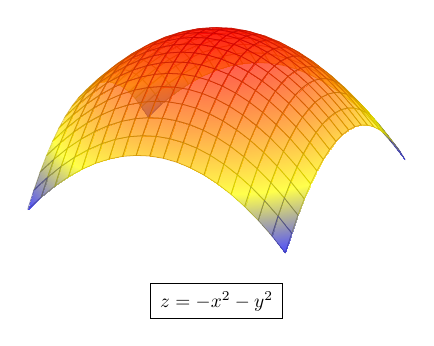
\begin{tikzpicture}[scale=0.7,trim axis left, trim axis right]
        \begin{axis}[
            hide axis,
            samples=20,
            legend cell align={left},
            legend style={at={(0.5, -0.05)},anchor=north},
            ]
            \addplot3[surf,shader=faceted interp, colormap/hot,opacity=0.7,domain=-1:1,y domain=-1:1,empty legend] {-x^2 - y^2};
            \addlegendentry{$z = -x^2 - y^2$};
        \end{axis}
        \end{tikzpicture}
        \captionof{figure}{Minimum point at $(0, 0)$.}
    \end{minipage}
    \medskip
    \tikzsetnextfilename{385}
    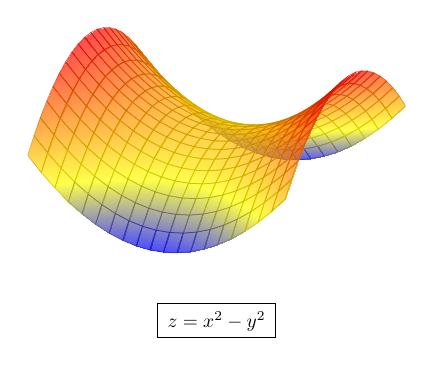
\begin{tikzpicture}[scale=0.7,trim axis left, trim axis right]
        \begin{axis}[
            hide axis,
            samples=20,
            legend cell align={left},
            legend style={at={(0.5, -0.05)},anchor=north},
            ]
            \addplot3[surf,shader=faceted interp, colormap/hot,opacity=0.7,domain=-1:1,y domain=-1:1,empty legend] {x^2 - y^2};
            \addlegendentry{$z = x^2 - y^2$};
        \end{axis}
    \end{tikzpicture}
    \captionof{figure}{Saddle point at $(0, 0)$.}
\end{figure}

\subsection{Global and Local Extrema}

In optimization, we may distinguish between a \vocab{local extremum} (a collective term used to refer to the maximum and minimum) from a \vocab{global extremum}. Basically, a global maximum/minimum is the highest/lowest value which the function can achieve.

Local extrema are like the stationary points which we just discussed. For example, consider the following graph of $f(x, y) = x\e^{-x^2-y^2}$:

\begin{figure}[H]\tikzsetnextfilename{386}
    \centering
    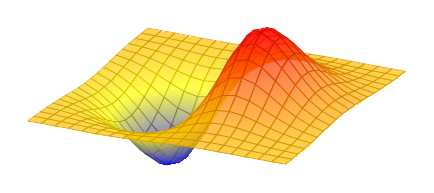
\begin{tikzpicture}[scale=0.7,trim axis left, trim axis right]
        \begin{axis}[
            hide axis,
            samples=20,
            ]
            \addplot3[surf,shader=faceted interp, colormap/hot,opacity=0.7,domain=-2:2,y domain=-2:2] {3 * x * e^(-x^2 - y^2)};
        \end{axis}
    \end{tikzpicture}
    \caption{}
\end{figure}

The intuitive idea behind local extrema is that when we move away from the maxima/minima in any direction, the value of the function will decrease/increase. However, this may not apply to global extrema. Consider the function $f(x, y) = x^2 + y^2$ with domain $-2 \leq x \leq 2$, $-2\leq y \leq 2$.

\begin{figure}[H]\tikzsetnextfilename{387}
    \centering
    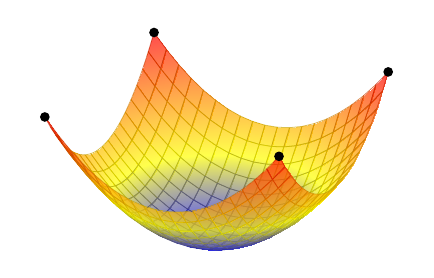
\begin{tikzpicture}[scale=0.7,trim axis left, trim axis right]
        \begin{axis}[
            hide axis,
            samples=20,
            xmax = 2.2,
            xmin = -2.2,
            ymax = 2.2,
            ymin = -2.2,
            ]
            \addplot3[surf,shader=faceted interp, colormap/hot,opacity=0.7,domain=-2:2,y domain=-2:2] {x^2+ y^2};
            \fill (-2, 2, 8) circle[radius=2.5pt];
            \fill (-2, -2, 8) circle[radius=2.5pt];
            \fill (2, 2, 8) circle[radius=2.5pt];
            \fill (2, -2, 8) circle[radius=2.5pt];
        \end{axis}
    \end{tikzpicture}
    \caption{}
\end{figure}

The global maxima occur at the corners of the domain. Note that these global maxima are also not stationary points.

\begin{recipe}[Finding Global Extrema]
    To find the global extrema of a function, we must
    \begin{itemize}
        \item check all local extrema (set $\nabla f = \vec 0$), and
        \item check for extrema along the boundary of the function's domain.
    \end{itemize}
\end{recipe}

\subsection{Second Partial Derivative Test}

We can determine the nature of the stationary points by the second partial derivative test:

\begin{proposition}[Second Partial Derivative Test]
    Let $(a, b)$ be a stationary point of $f(x, y)$. Let \[D = f_{xx}(a, b) f_{yy}(a,b) - \bs{f_{xy}(a, b)}^2.\]
    \begin{itemize}
        \item If $D > 0$, and
        \begin{itemize}
            \item $f_{xx}(a, b) > 0$ (or $f_{yy} (a, b) > 0$), then $(a, b)$ is a minimum point.
            \item $f_{xx}(a, b) < 0$ (or $f_{yy} (a, b) < 0$), then $(a, b)$ is a maximum point.
        \end{itemize}
        \item If $D < 0$, then $(a, b)$ is a saddle point.
        \item If $D = 0$, the test is inconclusive.
    \end{itemize}
\end{proposition}
The proof is similar to the proof of the second derivative test for univariate functions (see Proposition~\ref{prop:Second-Derivative-Test}).
\begin{proof}
    Consider the quadratic approximation $Q(x, y)$ of $f(x, y)$ at a stationary point $(a, b)$. We have $f_x(a, b) = f_y(a, b) = 0$, hence \[Q(x, y) = f(a, b) + \frac12 \bs{f_{xx} (a, b) (x-a)^2 + 2 f_{xy}(a, b) (x-a)(y-b) + f_{yy}(a, b) (y-b)^2}.\] Let \[P(x, y) = f_{xx} (a, b) (x-a)^2 + 2 f_{xy}(a, b) (x-a)(y-b) + f_{yy}(a, b) (y-b)^2.\] We can view $P(x, y)$ as a quadratic in $(x-a)^2$. Consider the discriminant $\D$ of $P(x, y)$:
    \begin{align*}
        \D &= \bs{2 f_{xy}(a, b) (y-b)}^2 - 4 f_{xx} (a, b) f_{yy}(a, b) (y-b)^2\\
        &= -4(y-b)^2 \bp{f_{xx}(a, b)f_{yy}(a, b) - \bs{f_{xy}(a, b)}^2}.
    \end{align*}
    Let $D = f_{xx}(a, b)f_{yy}(a, b) - \bs{f_{xy}(a, b)}^2$. We make the following observations:
    \begin{itemize}
        \item If $D > 0$, then $\D < 0$.
        \begin{itemize}
            \item If $f_{xx}(a, b) > 0$, then $P(x, y) > 0$ (since $f_{xx}(a, b)$ is the leading coefficient of $P(x, y)$). Thus, $Q(x, y) \geq f(a, b)$, whence $(a, b)$ is a minimum point.
            \item If $f_{xx}(a, b) < 0$, then $P(x, y) < 0$. Thus, $Q(x, y) \leq f(a, b)$, whence $(a, b)$ is a maximum point.
        \end{itemize}
        \item If $D < 0$, then $\D > 0$. This means that $P(x, y)$ has zeroes elsewhere other than $(a, b)$, and it is sometimes positive and negative. Hence, $(a, b)$ is a saddle point.
        \item If $D = 0$, then $\D = 0$. Hence, $P(x, y)$ has zeroes elsewhere other than $(a, b)$, and it is either always $> 0$ or $< 0$ outside the zeroes. Thus, the stationary point could be a maximum, a minimum or even a saddle point; the test is inconclusive.
    \end{itemize}
\end{proof}